\section{System composition and design details}

Darwinia ChainRelay has three key design schemes. The first is to use MMR to solve the scheme without uploading each block header. The second is to use MMR to verify the validity of the block without forking the target chain. Under the assumption of economic rationality, the system is optimized and optimized by using the Verification Game and the pledge incentive mechanism.

\subsection*{Chain Commitment}

In order to achieve the sub-linear property, we have to make sure that those provers commit their chain before further interaction, because the relay in our system won't download every node's head to achieve economic efficiency. If we don't ask for a commitment in advance, it will be difficult for a judge with limited computing power to efficiently locate the fork point of the two chains involved in potential disputes, because the malicious node can deceive the judge along with the erification game. Finding a invalid node will be much easier with a chain commitment.

The most basic and vital blockchain commitment data structure is the Merkle Tree. Bitcoin and its SPV clients have widely used Merkle Tree. In some other blockchain networks in the future, some changes in Merkle Tree have also occurred. Such as Merkle Patricia Tree and Merkle Mountain Range(MMR), etc. These variants have added some other useful features while maintaining the characteristics of the Merkle Tree. Here we will only introduce MMR, and the introduction about Merkle Tree and Merkle Patricia Tree is put in the appendix.

\subsubsection*{Merkle Mountain Range}

To submit the entire blockchain, Darwinia ChainRelay requires the prover to maintain a Merkle tree structure called Merkle Maintain Range (MMR) on all blocks added to the blockchain so far. In addition to Merkle trees, MMR also allows valid additions on the prover and valid block inclusion verification on the verifier. Also, it enables a valid subtree proof, that is, a proof that two MMRs are consistent on the first k leaves. At each block height i, the prover appends the hash of the previous block Bi-1 to the latest MMR and records the new MMR root Mi in the header of Bi (see Figure 1). As a result, each MMR root stored at each block height can be viewed as a commitment to the entire blockchain that reaches that height.

Merkle Mountain Range is a variant of the Merkle Tree data structure. Unlike Merkle Tree, MMR can quickly build new MMRs by adding leaf nodes to the existing tree structure incrementally. Below is an example of an MMR structure:

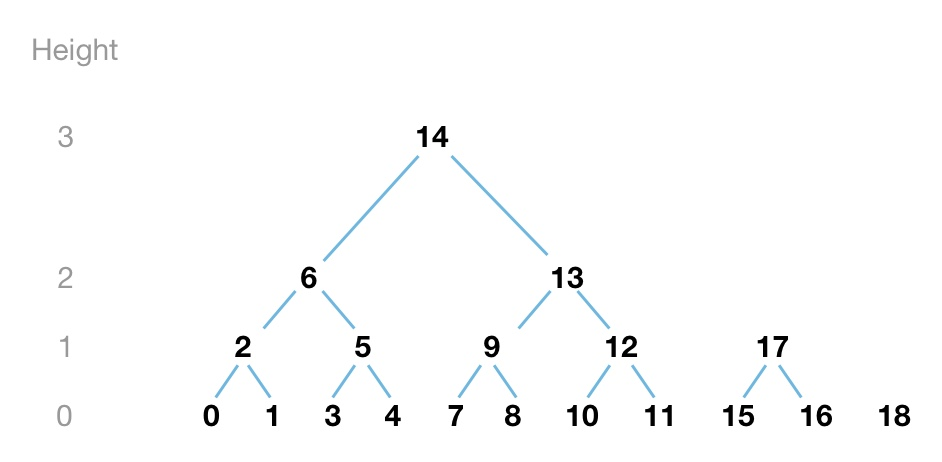
\includegraphics[scale=0.2]{pic/MMR1.jpg}

Here is a picture showing how to calculate root:

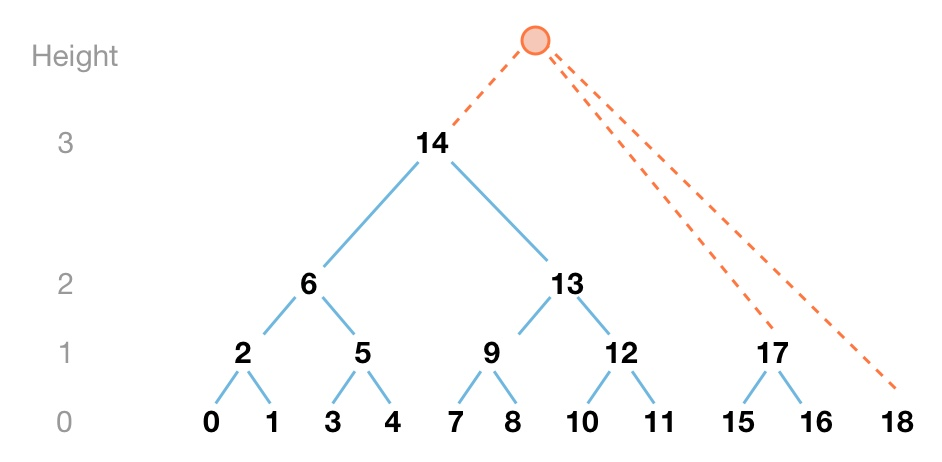
\includegraphics[scale=0.2]{pic/MMR2.jpg}

\textbf{definition}

A Merkle Mountain Range, M, is defined as a tree with n leaves, root r, and the following properties:

\begin{itemize}
    \item  M is a binary hash tree.
    \item M has depth ⌈log2 n⌉.
    \item \begin{verbatim}
If n>1, let n=2i +j such that i=⌊log2(n−1)⌋:
    - r.left is an MMR with 2i leaves.
    - r.right is an MMR with j leaves.
    \end{verbatim}

\end{itemize}

\textbf{Note}: M is a balanced binary hash tree, i.e., M is a Merkle tree. Therefore, for all nodes $k \in M$ , $\exists \Pi k \in M $.

\begin{theorem}
(Incremental) Given an MMR, M, with root r and n leaves, AppendLeaf(r,x) will return an MMR, M’, with $n+1$ leaves (the n leaves of M plus x added as the right-most leaf).
\end{theorem}

\begin{theorem}
(SubTree Root Generation) For $k \leq n$, given $\Pi xk  \in Mn$ , i.e., the Merkle proof that leaf xk is in Mn , a verifier can regenerate rk, the root of Mk. 
\end{theorem}

\begin{corollary}
(Chain Prefix Commit) If $x1,...,xn$ are the hashes of blocks 1 through n of chain Cn, rn commits the first n blocks to xn, and $\Pi k \in Mn$ for any k commits $x1,...,xk$ as the blocks of the chain Ck, where chain Ck is a prefix of chain Cn.
\end{corollary}

\begin{corollary}
(Block Commit) If an adversary changes any block i in the chain in any way, then its hash xi also changes, so any MMR Mk for $k \leq i$ with root rk' that contains the new block xi' has that $rk' /= rk$.
\end{corollary}

Darwinia ChainRelay is a sub-linear Relay, it cannot store all the blocks on the blockchain, and the verifier can trick the Relay by submitting a non-existing block certificate. To solve this problem, we need to append a new MMR root value to the latest block. At each block height i, the prover appends the hash of the previous block Bi-1 to the latest MMR and adds the new The MMR root Mi is recorded in the header of Bi. This MMR root value can be understood as a commitment to integrate the history of the blockchain. The prover of Darwinia ChainRelay can submit the block header and the MMR value together by maintaining the block header and its MMR value. (How to ensure the validity of the block header and MMR value is another issue, which we will solve by verifying the game protocol).

If MMR is applied to all block headers of the blockchain, that is, all block headers are used as leaf nodes of the MMR, the prover will be able to efficiently attach the MMR to the block header and push it to the light client or relay at the same time. With MMR, the verifier will be able to use the latest block MMR and verification block for efficient block inclusion proof, without requiring Relay to store all historical blocks. In addition, MMR can also be used for subtree proof, that is, the proof that two MMRs are consistent on the first k leaves.

The Merkle Mountain Range (MMR) model is an effectively updateable commitment mechanism that allows the prover to commit to the current blockchain with a small (constant size) commitment, and the inclusion proof of the block is logarithmic.


\subsubsection*{Chain Relay MMR Implementation}

To implement MMR in an ordinary light client, you need to make some modifications to the protocol, and add the MMR value as a part of the block header. But for Relay, which is a light client on the chain, there is some additional complexity in the implementation.

First, because the protocol of the target chain cannot be modified, the MMR value needs to be submitted to Relay as an addition to the block header, not as part of the block header. Second, suppose that we already know the Header and MMR values ​​of the previous block on the chain (in more complicated cases, we hand over the verification game protocol). When the Relay on the chain verifies the block header and its MMR, because we only have the MMR root Value, does not store the leaf nodes of all MMR blocks, so it is not possible to directly calculate the next block corresponding to the MMR tree from the previous MMR tree plus the next block header hash. In order to solve this problem, we divide it into two steps. First, calculate the MMR and its root value off-chain and submit the MMR root value to the chain. At the same time, the corresponding Merkle certificate of the previous block needs to be submitted. Second, after receiving the MMR root value on the chain, it is verified and passed. The Merkle proof of the block and the MMR root value is calculated to calculate the MMR root value of the previous block, and compared with the MMR value of the previous block submitted and verified before if they are consistent, the verification passes. In this way, it is not necessary to store the entire MMR tree corresponding to each block on the chain, but only the corresponding MMR root.


\subsection*{Verification Game}


\begin{figure*}
    \centering
    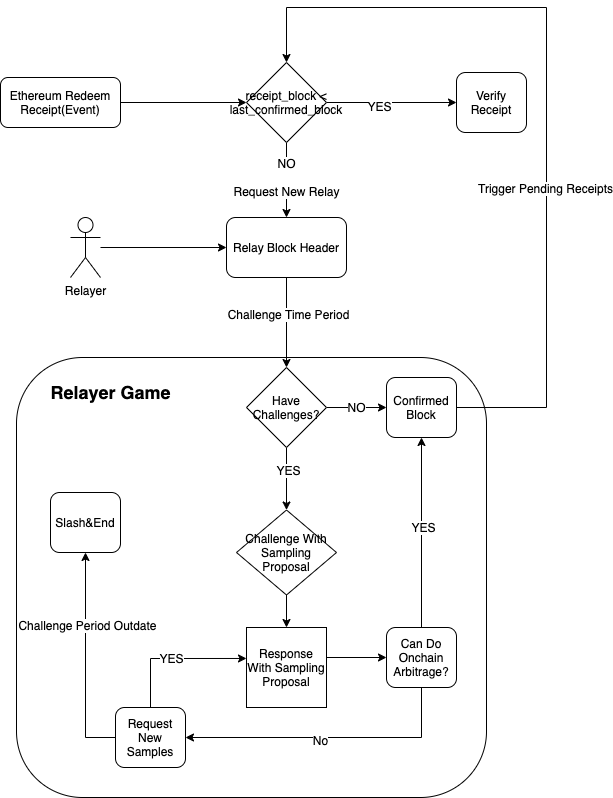
\includegraphics[scale=0.5]{pic/flowchart.png}
    \caption{FLowChart}
    \label{fig:my_label}
\end{figure*}

The goal of the interactive verification game is to provide a dispute resolution mechanism between the problem solver and the questioner, where the problem solver provides a solution to a computing problem, and the questioner does not agree with the solution, so Wake the verification game to achieve the purpose of the arbitration. This arbitration process is generally iterative and convergent.

The verification game protocol is used in Darwinia ChainRelay to solve the problem of attackers submitting illegal chains. The solution is to introduce economic games to make honest nodes motivated and have methods to find the wrong submissions and ensure the correctness of the state of light nodes And legitimacy. In order to introduce a verification game, two conditions are required. One is to have an incentive system and guarantee openness to attract enough honest participants to participate in it. The second is to prove honestly when an attacker submits wrong block data. The author can have a way to prove its error. Since the performance and economic feasibility of the verification and disapproval process must be considered, this process can be either one-time fast, iterative, and convergent. The process of iteration and convergence is acceptable because this affects the participants of the system to an optimal balance, that is, under the premise of economic rationality, most malicious people will not launch attacks.

The verification game will go through a series of rounds, each round reducing the scope of the controversial calculation. In the first round, the challenger forces the solver to perform a determined and timed pair of calculation steps. In the next round, the challenger repeatedly challenges a subset calculated by the solver during this interval, and then continues to challenge in a subset of the subset, and so on, until, in the final round, the final challenge becomes minor enough that the judges can make a final decision on whether the challenge is justified. The referee also requires the solver and challenger to follow the rules of the game. At the end of the verification game, either the cheating solver is found and punished in the outer layer of Darwinia ChainRelay, or the challenger pays the resources consumed by the false alarm.

\subsubsection*{Verification Protocol} 

With our actor’s model, which is mentioned at section III, we can describe a protocol process. If both prover nodes have submitted the same block header and block, and their chain heights are the same, the client can directly accept this submission, and this part of the agreement ends. Otherwise, if the data submitted by the two provers are inconsistent, it means that one of the provers holds an invalid chain. In this case, the system will use a sub-protocol called a verification game to determine which of the two provers submitted is the chain of honesty. 

\begin{itemize}
    \item Verifier has access to r = root of some Merkle tree, MT.
    \item The Prover has access to MT and generates a Merkle-Proof path of some $x \in MT = \Pi k \in MT$ using protocol 3 and sends it to the verifier.
    \item Verifier uses the proof and x to build up the path to r' using protocol 4, and checks that r' = r.
    \item If the checks pass, the Verifier accepts the proof, otherwise, it rejects the proof.
\end{itemize}

\subsubsection*{On-demand Verification Design}

According to the commonly used collaboration process in Chain Relay, Darwinia ChainRelay steps can be summarized as follows:

\begin{itemize}
    \item Step A: A prover (also known as Relayer or Worker) submits the block header and its MMR value to the on-chain relay.
    \item Step B: The on-chain relay performs the block header and MMR validity verification process. The central part includes a verification game protocol, and some other provers may participate in it.
    \item Step C: Relay on the chain determines the finality of the block header
    \item Step D: The verifier (also known as the verification service user) submits the transaction or receipt that needs to be verified to the chain, uses the MMR to prove the existence of the block and uses the corresponding Merkle tree root of the block header to conduct the existence proof of the transaction (receipt).
    \item Step E: Other on-chain operations performed after the cross-chain verification passes (or fails).
\end{itemize}

Even further, we can make some overall optimizations to this process, which can save unnecessary on-chain submission operations. Because the requirements generally come from steps D and E, we can improve and design a relay that the prover submits on demand, that is, the three operations A, B, and C are not scheduled or required for each block, but when the user executes step D and finds that the relevant block header and MMR certificate are missing, then A, B, and C operations are performed. The optimized steps are as follows:

\begin{center}
    $Verifier \longrightarrow Pre\_D \longrightarrow A \longrightarrow B \longrightarrow C \longrightarrow D \longrightarrow E$
\end{center}

\subsubsection*{Economic Incentive Model}

To ensure the decentralization and sustainability of the agreement, we need to design the agreement so that it does not require a license and introduces economic incentives so that the entire system can continue to run autonomously.

In Darwinia ChainRelay, the economic incentive model is mainly divided into the Relay framework layer and the verification game sub-protocol layer.
The former is a general economic model of Relayer. It is used to motivate the prover (also called Relayer or Worker) to submit block headers and MMRs to the system to maintain the Relay status and provide verification services to the verifier. In general, it is used to encourage proof The income of the verifier comes from the service fee paid by the verifier. For a specific Relayer, the corresponding Relayer status check must be completed. Therefore, the workload and cost of the prover to submit the block header and its MMR are relatively fixed, and the verification service The demand comes from the market and application needs. If the service revenue can be kept greater than the cost, we call the design of the Relayer economically feasible. For the traditional linear relayer, it is necessary to submit the block header to maintain the relayer state continuously to continuously submit the block header to maintain the relayer state, so the fuel cost is very high, and it is not economically feasible in many scenarios, such as BTCRelay. Darwinia ChainRelayer, as a sub-linear relay optimized by on-demand verification, can achieve good economic feasibility, and the verifier only needs to pay a small fee to complete cross-chain verification.

At the same time, Darwinia ChainRelay introduced a sub-protocol of the verification game to achieve a sub-linear relay. Therefore, in addition to the economic incentive design related to the relay, we also need to design a corresponding economic model for this verification game protocol. Because economic rationality is an essential premise for verifying game protocols, it is through mechanisms such as the Prove-or-punish introduced in the verification game that this hypothesis of economic rationality can work.

\subsubsection*{Relay Economic Incentive Model}

In the general relay, the prover is responsible for submitting the block header and its MMR to maintain the relay state, and the verifier uses the verification service provided by the relay. The prover can be anyone, but the submission of the block header and its MMR is not free, and network fees need to be paid. To ensure that enough certifiers are willing to participate in it, maintain a competitive market, and be sustainable, verify the pricing of services There is a need to provide a premium above the average cost level. For the traditional linear relay, a simplified way is to calculate and accumulate all the block submission costs and accumulate them into a cost contribution pool. When providing verification services, use the average level of the cost contribution pool in the past as a reference. Under this model, because the use of future verification services is difficult to predict, the price of verification services will continue to fluctuate, and the contribution of the workload provided by the prover will be at risk of making ends meet.

\begin{center}
Price of verification service = (cumulative fuel fee submitted by the block header within T / number of times verification service is used) + premium

Because Darwinia ChainRelay has the optimization of on-demand verification, the cost of its verification service is also simplified, so this model can be simplified to:

Verification service price = block header submission fuel fee + premium
    
\end{center}

The optimization of on-demand verification has two benefits. The first benefit is that before using the verification service, you can determine the price of the verification service and decide whether to continue using the verification service. If you do not continue, you do not need to submit the block header, and the prover does not need to submit the block header, so you do not need to pay for fuel costs, which reduces waste. It can be seen that in this case, because the prover has no risk of making ends meet, anyone is willing to participate in it if they have the ability. The second benefit is that because the cost of submitting the fuel fee for the block header will not change significantly, and under the condition of sufficient competition, the premium will also be very meager low, so it can continue to provide more stable verification service prices.

\subsubsection*{Verification Game Economic Model}

In Darwinia ChainRelay, after the prover submits a block header and MMR value because its previous block header status is generally not submitted or unknown, it cannot be immediately determined whether it is valid or not. Observer A in the figure below might be the first submitter, but after entering the verification game protocol, it is impossible to determine whether each observer is honest until it has wholly converged, until a block header record that has been submitted is the most recent The block header to be verified is the previous one. In this case, we use the Pre\_Hash and MMR subtree theorem to determine the validity of the submitted block header.


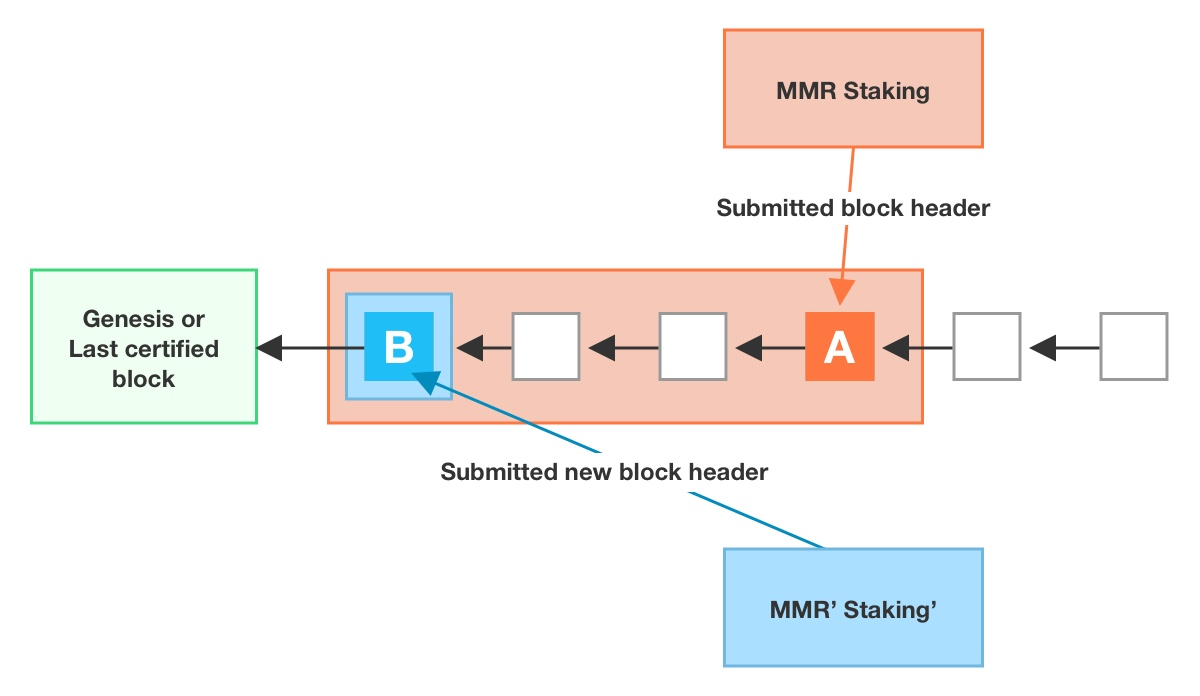
\includegraphics[scale=0.2]{pic/Verification Game Economic Model 1.jpg}


In the whole process, the design goal of the pledge punishment system is to make the verification game agreement end as soon as possible, so as to achieve the effect and equilibrium of the optimistic verification game. Therefore, when each challenge observer further advances the verification game process by submitting a new block header, a fixed value pledge is required to be locked in the protocol. After the convergence is judged, the honestly submitted pledge will be returned but the collateral submitted by the fraud challenger will be confiscated by the system. These confiscated materials can be used to reward the winner of the final verification game process, that is, the honest prover. We have previously proven that honest provers must win the verification game process.

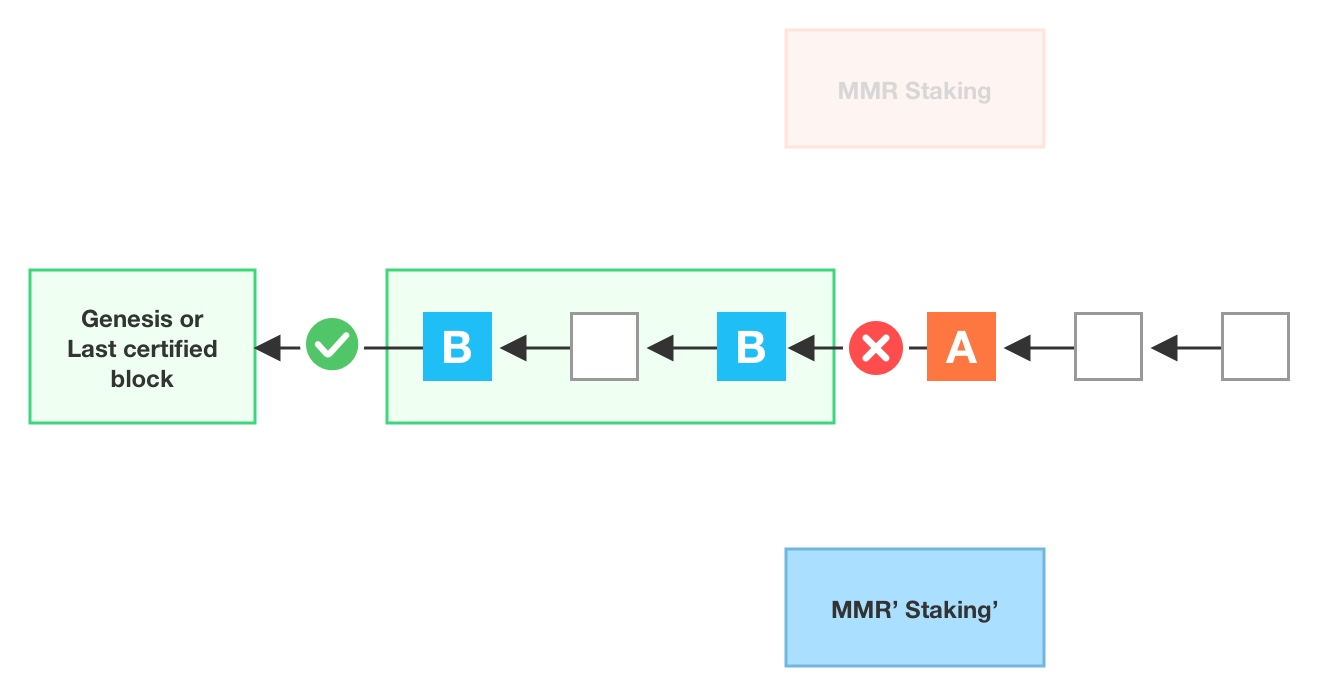
\includegraphics[scale=0.19]{pic/Verification Game Economic Model 2.jpg}

In the above verification game harvesting process, the process of submitting the pledged items for confiscation and winning back is gradually progressive (recursive). In the simplified case, there may only be two observers and opponents playing against each other, but the more complex multi-party game situation is also possible, so during the submission and challenge, the opponent relationship between the players will be recorded. The last submitter of the challenge is the opponent of the challenger, and the pledged items confiscated after the failure of the opponent will be returned to another party. The figure above shows the process of the pledge of the fraud prover being gradually harvested by the honest prover.

It can be seen that once entering the verification game protocol, the attack cost of the fraud prover is very high, and it is proportional to the time of the attack, and the benefit of the honest challenger is very considerable, and multiple honest challengers can cooperate and work together to fight against the fraud prover, the pledge of the fraud prover will be confiscated and rewarded to the honest challenger.


\subsubsection*{Optimistic Behavior Analysis}

The above verification game seems to have a disadvantage. Once it enters the verification game, although it is convergent, its time-consuming may be very long. However, after further analysis, we found that if the assumption of economic rationality is introduced, due to the punishment and incentive mechanism, the attacker is not willing to enter the verification game process because the game participation is sufficiently open. Eyeing enters the verification game, and the perpetrators will eventually fail with certainty, and be punished for bearing the attack losses. Because the process of verifying the game can be participated by anyone, it is only necessary to have at least one honest challenger (monitor) to ensure that the final block confirmed by Darwinia ChainRelay is legal. For economically rational participants, it is impossible to attack, because the attack has no possibility of reward or success, but it may bear the penalty of forfeiture. Therefore, it can be concluded that the vast majority of the solutions provided by the solver are correct, and no subsequent verification process will be performed. The block header and the MMR submitted by the solver will be deleted after a short challenge waiting period. confirm. Only a small number of unintentional procedural errors may enter the short-term verification game process. Participating in an unintentional error cannot be discerned whether it is intentional and affects system reliability, so it will also be punished.

\textbf{DOS} If we assume that the attacker is non-economically rational and willing to pay a certain cost to attack the system, then Delay Confirmation attacks will be a more common type, that is, the attacker pays the price of the pledged fee for the penalty to extend the verification game as a result, a block header in Darwinia ChainRelay, namely its MMR, cannot be confirmed for a long time. However, it is worth noting that its attack cost is linearly related to its Delay Confirmation attack effect (time duration), so it can be suppressed by adjusting the penalty parameter, and this theoretical possibility exists in many networks, which is not a severe issue.

\subsubsection*{Put Things Together}


With the help of MMR and verification game protocols, we can assemble a sub-linear Relay on the chain to provide cross-chain verification services. The Relay on the chain stores the discontinuous block header and its derived MMR value. This value is submitted by the prover and verified and verified by the verification game protocol. There is a premise that at least one honest prover participates in the Agreement process.

When a block header and its MMR value are stored and confirmed by the relay on the chain, then the validator can use this valid information of the relay for cross-chain verification, and the validator can verify any transaction or receipt before the block is changed. 

